\documentclass{standalone}
\usepackage{tikz}
\usepackage{amssymb}
\usetikzlibrary{automata, positioning}

\begin{document}
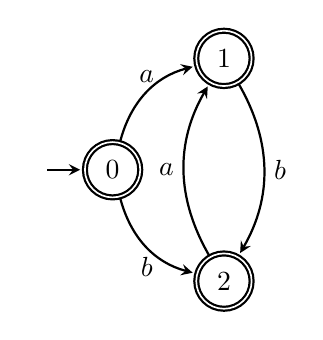
\begin{tikzpicture}[%
    >=stealth,
    shorten >=1pt,
    node distance=2cm,
    on grid,
    auto,
    state/.append style={minimum size=2em},
    thick
  ]

  \node[state, initial, initial text = {}, accepting] (A) {$0$};
  \node[state, accepting] (B) [above right of=A] {$1$};
  \node[state, accepting] (C) [below right of=A] {$2$};
  \path[->] 
            (A) edge [bend left] node[above]{$a$} (B)
            (A) edge [bend right] node[below] {$b$} (C)
            (B) edge [bend left] node {$b$} (C)
            (C) edge [bend left] node {$a$} (B);
\end{tikzpicture}
\end{document}